\documentclass[
	12pt, 
	a4paper, 
	openright, 
	twoside
]{abntex2}                                                                          % modelo abntex2(memoir). Fonte 12, papel A4, twoside(ambos lados) e openright(anverso) para elementos pré textuais e novos chapters
% \usepackage{helvet}                                                                 % pacote helvet/arial
% \renewcommand{\familydefault}{\sfdefault}                                           % configura fonte como serif (Arial)
\usepackage[T1]{fontenc}                                                            % fonte
\usepackage[utf8]{inputenc}                                                         % codificação do arquivo tex, caracteres utf8
\usepackage[brazil]{babel}                                                          % hifenização
% \usepackage{sectsty}                                                                % formatação de seções
% \sectionfont{\clearpage}                                                            % nova página para cada seção 
% \usepackage[a4paper,top=3cm,left=3cm,right=2cm,bottom=2cm]{geometry}                % bordas
\PassOptionsToPackage{hyphens}{url}\usepackage{hyperref}                            % formatação de url's e hyperlink neles
% \usepackage[alf, abnt-emphasize=bf]{abntex2cite}                                    % citações estilo ABNT, opção [alf] para citação (autor, data) e [num,overcite] para citação estilo [1]. abnt-emphasize=bf para deixar títulos em negrito https://linorg.usp.br/CTAN/macros/latex/contrib/abntex2/doc/abntex2cite.pdf

\usepackage[num,overcite]{abntex2cite}                                              % citações estilo ABNT, opção [alf] para citação (autor, data) e [num,overcite] para citação estilo [1]. https://linorg.usp.br/CTAN/macros/latex/contrib/abntex2/doc/abntex2cite.pdf
\citebrackets[]																		% estilo de colchetes para as fontes
% \usepackage[nottoc]{tocbibind}                                                      % opções do sumário, bibliografia no sumário, tirar autorreferência ao sumário 
\usepackage{graphicx}                                                               % imagens e gráficos graphviz
\usepackage{tikz}                                                                   % imagens tikz, usado com dot2tex
\usepackage{amsmath}                                                                % equações
\usepackage{mathtools}                                                              % mais símbolos matemáticos
\usepackage{amssymb}                                                                % símbolos, como flechas e outros
\usepackage{mathrsfs}                                                               % símbolos extras com comando \mathscr, ex: símbolos para transformadas F, Z e L
\usepackage{siunitx}                                                                % unidades SI
\usepackage{indentfirst}                                                            % identar primeira linha depois do comando \section ou \subsection
\usepackage{xcolor}                                                                 % definição de cores, usado na listagem de código
% \renewcommand{\arraystretch}{1.7}                                                   % separação vertical entre células em tabelas
\usepackage{pdfpages}                                                               % inclusão de pdf's

\usepackage{luacode}                                                                % macros para melhor execução de código lua, \luaexec e \begin{luacode} ... \end{luacode}. https://linorg.usp.br/CTAN/macros/luatex/latex/luacode/luacode.pdf
\usepackage{luapackageloader}                                                       % pra máquina lua procurar pacotes nos paths
\directlua{package.path = "./lua/?.lua;" .. package.path }             % anexa o meu path do lua rocks pra pacotes no package.path, mudar se necessário

% comandos para usar no tabular de forma a dar tamanho para as colunas, util para dar espaço extra ou realizar quebra de texto dentro das células. Ex: \begin{tabular}{|cC{2cm}L{4cm}r|}
% left fixed width:
\newcolumntype{L}[1]{>{\raggedright\arraybackslash}p{#1}}
% center fixed width:
\newcolumntype{C}[1]{>{\centering\arraybackslash}p{#1}}
% flush right fixed width:
\newcolumntype{R}[1]{>{\raggedleft\arraybackslash}p{#1}}

% Listagem de código fonte
\usepackage{listings}

\makeatletter
\lst@Key{source}{}{\def\lst@source{#1}} % adicionar opção de fonte
\lst@Key{sourcePrefix}{}{\def\lst@sourcePrefix{#1}} % adicionar opção de prefixo da fonte. Ex: 'Fonte: '

\let\orig@lst@MakeCaption=\lst@MakeCaption % redefinir comando de caption para códigos
\def\lst@MakeCaption#1{%
    \orig@lst@MakeCaption#1%
    \ifx b#1%
        \ifx\lst@source\@empty\else
            \noindent
            \vskip\belowcaptionskip
            \expandafter\lst@makesourcebox\expandafter{\lst@sourcePrefix{} \lst@source{}}%
        \fi
    \fi
}

\def\lst@makesourcebox#1{ % caixa para receber a legenda inferior da fonte
    \makebox[\linewidth][c]{
        \fontfamily{\familydefault}\selectfont
        \footnotesize #1
    }%
}
\makeatother

% estilo da listagem de código
\definecolor{background_color}{HTML}{f8f8fd}
\definecolor{comment_color}{HTML}{6AAF19}
\definecolor{keyword_color}{HTML}{F92672}
\definecolor{ndkeyword_color}{HTML}{00FF00}
\definecolor{string_color}{HTML}{F25A00}
\definecolor{identifier_color}{HTML}{000000}
\definecolor{line_number_color}{HTML}{000000}
\lstdefinestyle{mystyle}{
    backgroundcolor=\color{background_color},   
    commentstyle=\color{comment_color},
    keywordstyle=\color{keyword_color},
    ndkeywordstyle=\color{ndkeyword_color},
    numberstyle=\tiny\color{line_number_color},
    stringstyle=\color{string_color},
    identifierstyle=\color{identifier_color},
    basicstyle=\ttfamily\footnotesize,
    breakatwhitespace=false,         
    breaklines=true,                 
    keepspaces=true,                 
    numbers=left,                    
    numbersep=5pt,                  
    showspaces=false,                
    showstringspaces=false,
    showtabs=false,                  
    tabsize=2,
    captionpos=t,
    aboveskip=15pt,
    belowskip=15pt,
    belowcaptionskip=1ex,
    xleftmargin=1em,
    numbersep=0.5em,
    numberbychapter=false
}
\renewcommand\lstlistingname{Código}
\renewcommand\lstlistlistingname{Códigos}
\lstset{style=mystyle}                                                              % definir estilo de código

% estilo memoir de list, para fazer uma lista de listings
% https://tex.stackexchange.com/a/27648
\begingroup\makeatletter
\let\newcounter\@gobble\let\setcounter\@gobbletwo
	\globaldefs\@ne \let\c@loldepth\@ne
	\newlistof{listings}{lol}{\lstlistlistingname}
	\newlistentry{lstlisting}{lol}{0}
\endgroup
\renewcommand{\cftlstlistingname}{Código\space}
\renewcommand*{\cftlstlistingaftersnum}{\hfill\textendash\hfill}
\newcommand{\listoflistings}{\begin{KeepFromToc}\lstlistoflistings{}\end{KeepFromToc}}

\def\UrlLeft{}                                                                      % tira o sinal < na frente das URLs
\def\UrlRight{}                                                                     % tira o sinal > depois das URLs

\renewcommand{\legend}[1]{                                                          % definir prefixo para comando de legenda de fonte que fica em baixo de figuras e tabelas
    \par
    \centering
    \fontfamily{\familydefault}\selectfont 
    \footnotesize Fonte: #1
}	
\setFloatSpacing{1}																	% espaçamento entre linhas em elementos float(imagens, tabelas e outros) para a legenda e fonte 

\setlength{\cftbeforefigureskip}{0.75ex}                                             % espaçamento de 1.5 na lista de figuras
\setlength{\cftbeforetableskip}{0.75ex}                                              % espaçamento de 1.5 na lista de tabelas

% chapter font config
\renewcommand{\ABNTEXchapterfont}{\fontseries{bx}\fontshape{n}\selectfont}          % estilo da fonte, negrito, não itálico, maiúsculo, tamanho 12pt (\normalsize)
\setboolean{ABNTEXupperchapter}{true}          										
\renewcommand{\ABNTEXchapterfontsize}{\normalsize}         							
\setlength{\beforechapskip}{1.5ex}													% espaçamento entre titulo do capitulo e o paragrafo anterior de aproximadamente 1.5
\setlength{\afterchapskip}{1.5ex}													% espaçamento entre titulo do capitulo e o paragrafo seguinte de aproximadamente 1.5
\setlength{\cftbeforechapterskip}{0.75ex}         									% espaçamento de 1.5 no sumário
\renewcommand{\cftchapterfont}{\ABNTEXchapterfont}                  				% definir mesmo estilo de fonte no sumário
\renewcommand{\cftchapterpagefont}{\cftchapterfont}

% part font config
\renewcommand{\ABNTEXpartfont}{\fontseries{bx}\fontshape{n}\selectfont}             % estilo da fonte, negrito, não itálico, maiúsculo, tamanho 12pt (\normalsize)
% \setboolean{ABNTEXupperpart}{false}            										
\renewcommand{\ABNTEXpartfontsize}{\normalsize}            							
% \setlength{\beforepartskip}{1.5ex}													% espaçamento entre titulo da parte e o paragrafo anterior de aproximadamente 1.5
% \setlength{\afterpartskip}{1.5ex}													% espaçamento entre titulo da parte e o paragrafo seguinte de aproximadamente 1.5
% \setlength{\cftbeforepartskip}{1.5ex}            									% espaçamento de 1.5 no sumário
% \renewcommand{\cftpartfont}{\ABNTEXpartfont}                        				% definir mesmo estilo de fonte no sumário
% \renewcommand{\cftpartpagefont}{\cftpartfont}

% section font config
\renewcommand{\ABNTEXsectionfont}{\fontseries{m}\fontshape{n}\selectfont}           % estilo da fonte, não negrito, não itálico, maiúsculo, tamanho 12pt (\normalsize)
\setboolean{ABNTEXuppersection}{true}          										
\renewcommand{\ABNTEXsectionfontsize}{\normalsize}  
\setlength{\beforesecskip}{1.5ex}													% espaçamento entre titulo da seção e o paragrafo anterior de aproximadamente 1.5
\setlength{\aftersecskip}{1.5ex}       												% espaçamento entre titulo da seção e o paragrafo seguinte de aproximadamente 1.5
\setlength{\cftbeforesectionskip}{0.75ex}         									% espaçamento de 1.5 no sumário
\renewcommand{\cftsectionfont}{\ABNTEXsectionfont}                  				% definir mesmo estilo de fonte no sumário
\renewcommand{\cftsectionpagefont}{\cftsectionfont}

% subsection font config
\renewcommand{\ABNTEXsubsectionfont}{\fontseries{b}\fontshape{n}\selectfont}        % estilo da fonte, negrito, não itálico, minúsculo, tamanho 12pt (\normalsize)
\setboolean{ABNTEXuppersubsection}{false}      										
\renewcommand{\ABNTEXsubsectionfontsize}{\normalsize}      
\setlength{\beforesubsecskip}{1.5ex}   												% espaçamento entre titulo da sub seção e o paragrafo anterior de aproximadamente 1.5
\setlength{\aftersubsecskip}{1.5ex}    												% espaçamento entre titulo da sub seção e o paragrafo seguinte de aproximadamente 1.5
\setlength{\cftbeforesubsectionskip}{0.75ex}      									% espaçamento de 1.5 no sumário
\renewcommand{\cftsubsectionfont}{\ABNTEXsubsectionfont}            				% definir mesmo estilo de fonte no sumário
\renewcommand{\cftsubsectionpagefont}{\cftsubsectionfont}

% subsubsection font config
\renewcommand{\ABNTEXsubsubsectionfont}{\fontseries{m}\fontshape{n}\selectfont}    % estilo da fonte, não negrito, itálico, minúsculo, tamanho 12pt (\normalsize)
\setboolean{ABNTEXuppersubsubsection}{false}   										
\renewcommand{\ABNTEXsubsubsectionfontsize}{\normalsize}   
\setlength{\beforesubsubsecskip}{1.5ex}												% espaçamento entre titulo da sub sub seção e o paragrafo anterior de aproximadamente 1.5
\setlength{\aftersubsubsecskip}{1.5ex} 												% espaçamento entre titulo da sub sub seção e o paragrafo seguinte de aproximadamente 1.5
\setlength{\cftbeforesubsubsectionskip}{0.75ex}   									% espaçamento de 1.5 no sumário
\renewcommand{\cftsubsubsectionfont}{\ABNTEXsubsubsectionfont}      				% definir mesmo estilo de fonte no sumário
\renewcommand{\cftsubsubsectionpagefont}{\cftsubsubsectionfont}

% nome de seção em maiúsculo no sumário
% https://tex.stackexchange.com/a/399861
\makeatletter
\let\oldcontentsline\contentsline
\def\contentsline#1#2{%
	\expandafter\ifx\csname l@#1\endcsname\l@section
		\expandafter\@firstoftwo
	\else
		\expandafter\@secondoftwo
	\fi
	{%
		\oldcontentsline{#1}{\MakeTextUppercase{#2}}%
	}{%
		\oldcontentsline{#1}{#2}%
	}%
}
\makeatother

% ajustes para anexo maiúsculo no sumário, no caso de Sumario (TOC) especifico da ABNT-6027-2012 precisa desse debaixo pro anexo ficar minúsculo
% \makeatletter
% \ifthenelse{\boolean{ABNTEXsumario-abnt-6027-2012}}{
% \settocpreprocessor{chapter}{%
%     \let\tempf@rtoc\f@rtoc%
%     \def\f@rtoc{%
%         \texorpdfstring{\MakeTextUppercase{\tempf@rtoc}}{\tempf@rtoc}}%
% }
% \settocpreprocessor{part}{%
%     \let\tempf@rtoc\f@rtoc%
%     \def\f@rtoc{%
%         \texorpdfstring{\MakeTextUppercase{\tempf@rtoc}}{\tempf@rtoc}}%
% }
% \settocpreprocessor{subsection}{%
%     \let\tempf@rtoc\f@rtoc%
%     \def\f@rtoc{%
%         \texorpdfstring{\MakeTextUppercase{\tempf@rtoc}}{\tempf@rtoc}}%
% }
% }{}
% \makeatother

% citação direta
\setlength{\ABNTEXcitacaorecuo}{4cm}

\renewenvironment{citacao}{
\begin{flushright}
\begin{SingleSpace}
\begin{minipage}{\textwidth - \ABNTEXcitacaorecuo + \foremargin}
\ABNTEXfontereduzida
}{      
\hspace{0.05\textwidth}
\end{minipage}
\end{SingleSpace}
\end{flushright}
}

\setlength{\ABNTEXsignwidth}{8.5cm}                                                 % largura da assinatura na folha de aprovação

\OnehalfSpacing                                                                     % espaçamento entre linhas

\counterwithout{equation}{chapter}                                                  % não enumerar equações por capitulo, fazer de forma contínua por todo o documento 

% https://linorg.usp.br/CTAN/macros/latex/contrib/memoir/memman.pdf#page=83
\captionnamefont{\ABNTEXfontereduzida}                                              % tamanho das legendas
\captiontitlefont{\ABNTEXfontereduzida}                                             % tamanho das legendas

% tipo de página, cabeçalho só mostra o número da página
\makepagestyle{simple-folio}
\makeevenhead{simple-folio}{\ABNTEXfontereduzida\thepage}{}{}
\makeoddhead{simple-folio}{}{}{\ABNTEXfontereduzida\thepage}
\directlua{require("lua/tablecsv.lua")}

% open file to be used by subsequent calls
% arg1: filename
\newcommand\openfile[1]{\luaexec{openFile(\luastring{#1},",",true)}}

% get a field value by col row reference
% arg1: col
% arg2: row
\newcommand\getfield[2]{\luaexec{getField(#1,#2)}}

% get a range from the opened file formatted for tex tabular's. Ex: "1 & 2 & 3 \\\hline"
% arg1: first col
% arg2: first row
% arg3: second col
% arg4: second row
\newcommand\tabularfromrange[4]{\luaexec{tabularFromRange(#1,#2,#3,#4)}}
% arg5: line ending. If not provided defaults to "\hline"
% \newcommand\getrange[5]{\luaexec{getRange(#1,#2,#3,#4,\luastring{#5})}}

%%%%%%%%%%%%%%%%%%%%%%%%%%%%%%%%%%%%%%%%%%%%%%%%%%%%%%%%%%%%%%%%%%%%%%%%%%%%%%%%%%%%%%%%%%%%%%%%

\titulo{TITULO}              								% titulo do trabalho
\autor{DISCENTE}                 							% nome do discente
\local{LOCAL}	               								% local/cidade
\def\estado{ES}												% estado, formato duas letras. Ex: SC, PR, SP 
\data{Outubro de 20XX}       								% data da capa
\def\Data{XX de XXXXXX de 202X}                      		% data da folha de aprovação
\def\instituicaoartigo{da}									% artigo para se referir a instituição. Ex: 'da' Universidade, 'do' Instituto
\def\nomeinstituicao{Universiade TAL/ Instituto TAL}		% nome da instituição
\def\curso{Bacharelado em CURSO}							% curso. Ex: Bacharelado em XXX, Licenciatura em XXXX
\def\cursotitulo{Bacharel em CURSO}							% titulo a quem se forma no curso. Ex: Bacharel em XXXX
\def\campus{Campus \imprimirlocal}							% campus. Ex: Campus Luzerna
\instituicao{ 												% instituição, curso e campus
	\nomeinstituicao
	\par
	\curso
	\par
	\textit{\campus}
}

\tipotrabalho{Trabalho de conclusão (Bacharelado)} 			% tipo de trabalho, usado na ficha catalográfica Ex: Trabalho de conclusão (Bacharelado), Tese (Doutorado), Dissertação (Mestrado).
\orientador{Prof. Msc. NOME} 								% nome do orientador
% \coorientador{Prof. Msc. NOME} 							% nome do coorientador
\def\primeiroavaliador{Prof. Msc. XXXXXXX}           		% primeiro avaliador
\def\primeiroavaliadorafiliacao{							% instituição do primeiro avaliador
	Universiade TAL/ Instituto TAL
}           		
\def\segundoavaliador{Prof. Dr. XXXXXX}              		% segundo avaliador
\def\segundoavaliadorafiliacao{								% instituição do segundo avaliador
	Universiade TAL/ Instituto TAL
}           		
\def\PalavrasChave{	                                 		% palavras chave para o resumo
	palavra-chave; palavra-chave; palavra-chave.
} 
\def\Keywords{												% palavras chave para o resumo em inglês
	keyword 1; keyword 2; keyword 3.
}
\preambulo{													% O preambulo deve conter o tipo do trabalho, o objetivo, o nome da instituição e a área de concentração 
	Trabalho de conclusão apresentado à banca examinadora do curso de \curso, do \nomeinstituicao, \campus, como requisito para a obtenção do título de \cursotitulo, em cumprimento às exigências de sua componente curricular.
}

%%%%%%%%%%%%%%%%%%%%%%%%%%%%%%%%%%%%%%%%%%%%%%%%%%%%%%%%%%%%%%%%%%%%%%%%%%%%%%%%%%%%%%%%%%%%%%%%
\renewcommand{\imprimircapa}{
	\begin{capa}
		\center
		\begin{figure}[!ht]
	        \centering
	        
\includegraphics[width = 0.25\textwidth]{images/logo.png}
        \end{figure}
        
		\imprimirinstituicao
    
		\vspace*{2cm}
    
		\textbf{{\ABNTEXchapterfont\normalsize\imprimirautor}}

		\vfill
		\begin{center}
			\ABNTEXchapterfont\bfseries\normalsize\imprimirtitulo
		\end{center}
    		\vspace*{2cm}
		\vfill

		\large\imprimirlocal

		\large\imprimirdata
    
		%\vspace*{1cm}
	\end{capa}
}
\makeindex
\begin{document}
\pretextual
\imprimircapa
\begin{folhadeaprovacao}

  \begin{center}
    \textbf{{\ABNTEXchapterfont\normalsize\imprimirautor}}

    \vspace*{\fill}\vspace*{\fill}
    \begin{center}
      \ABNTEXchapterfont\bfseries\normalsize\imprimirtitulo
    \end{center}
    \vspace*{\fill}
    
    \hspace{.45\textwidth}
    \begin{minipage}{.5\textwidth}
        \imprimirpreambulo
        
        Orientador: \imprimirorientador
    \end{minipage}%
    \vspace*{\fill}
   \end{center}

      
   \begin{center}
    \vspace*{0.5cm}
    {\large\imprimirlocal}
    \par
    {\large\imprimirdata}
    \vspace*{1cm}
  \end{center}
  
\end{folhadeaprovacao}
% Isto é um exemplo de Folha de aprovação, elemento obrigatório da NBR
% 14724/2011 (seção 4.2.1.3). Você pode utilizar este modelo até a aprovação
% do trabalho. Após isso, substitua todo o conteúdo deste arquivo por uma
% imagem da página assinada pela banca com o comando abaixo:

% \includepdf{folhadeaprovacao_final.pdf}

\begin{folhadeaprovacao}
\DoubleSpacing
\begin{center}

	{\ABNTEXchapterfont\imprimirautor}

	\vfill

	{\ABNTEXchapterfont\imprimirtitulo}

	\vspace*{1cm}

	\hspace{.45\textwidth}
	\begin{minipage}{.5\textwidth}
	\begin{SingleSpace}
		\imprimirpreambulo
	\end{SingleSpace}
	\end{minipage}

	\vspace*{1.5cm}
	
	\imprimirlocal ~(\estado), \Data :
	
	\assinatura{\textbf{\imprimirorientador} \\ \nomeinstituicao}
	
	\vspace*{1.5cm}
	\textbf{BANCA EXAMINADORA}

	\assinatura{\textbf{\primeiroavaliador}\\ \primeiroavaliadorafiliacao}
	\assinatura{\textbf{\segundoavaliador}\\ \segundoavaliadorafiliacao}	
\end{center}
\end{folhadeaprovacao}
\begin{dedicatoria}
\vspace*{\fill}
Exemplo: Este trabalho é dedicado aos meus colegas de classe, aos meus queridos pais e professores
\end{dedicatoria}

\begin{agradecimentos}
	Inserir os agradecimentos aos colaboradores à execução do trabalho.
\end{agradecimentos}
\begin{epigrafe}
\vspace*{\fill}
\hspace{.45\textwidth}
\begin{minipage}{.5\textwidth}
\itshape
	
	Texto da Epígrafe. Citação relativa ao tema do trabalho. É opcional. A epígrafe pode também aparecer na abertura de cada seção. Deve ser elaborada de acordo com a NBR 10520. \\

	\begin{flushright}		
	(SOBRENOME do autor da epígrafe, ano) 
	\end{flushright}
\end{minipage}
\end{epigrafe}
\setlength{\absparsep}{18pt} % ajusta o espaçamento dos parágrafos do resumo
\begin{resumo}
O texto do resumo em língua portuguesa deve ser digitado em um único bloco, sem espaço de parágrafo. O resumo deve ser significativo, composto de uma sequência de frases concisas, afirmativas e não de uma enumeração de tópicos. Não deve conter citações. O espaçamento entre linhas é 1,5 e o tamanho da fonte é 12. Abaixo do resumo deve-se informar as palavras-chave (palavras ou expressões significativas retiradas do texto) ou, termos retirados de thesaurus da área. De 150 a 500 palavras.
	
\textbf{Palavras-chave}: \PalavrasChave.
\end{resumo}

\begin{resumo}[Abstract]
\begin{otherlanguage*}{english}
O texto do resumo em língua inglesa deve ser digitado em um único bloco, sem espaço de parágrafo. O resumo deve ser significativo, composto de uma sequência de frases concisas, afirmativas e não de uma enumeração de tópicos. Não deve conter citações diretas. Abaixo do resumo deve-se informar as palavras-chave (palavras ou expressões significativas retiradas do texto) ou, termos retirados de thesaurus da área. Até 500 palavras.
 
\textbf{Keywords}: \Keywords.
\end{otherlanguage*}
\end{resumo}
\pdfbookmark[0]{\listfigurename}{lof}						% lista de ilustrações
\listoffigures*
\cleardoublepage

\pdfbookmark[0]{\listtablename}{lot} 						% lista de tabelas
\listoftables*
\cleardoublepage

\begin{siglas}												% lista de abreviaturas e siglas
    \item[TA]               Trabalho Acadêmico
	\item[$\omega _n $]     Ômega
	\item[$\varphi $]       Vetor Fi
	\item[$\Theta $]        Vetor Teta
	\item[Z]                Zeros
\end{siglas}

\begin{simbolos}											% lista de símbolos
	\item[$\xi $]           Coeficiente de amortecimento
    \item[$\Theta  _n $]    Enésimo ângulo
	\item[rad/s]            Radianos por segundo
	\item[s]                Segundo
    \item[j]                Variável imaginária
    \item[s]	            Variável laplaciana para sistemas contínuos
    \item[z]                Variável z para sistemas discretos
\end{simbolos}

\pdfbookmark[0]{\contentsname}{toc}  						% sumario
\tableofcontents*
\cleardoublepage
%%%%%%%%%%%%%%%%%%%%%%%%%%%%%%%%%%%%%%%%%%%%%%%%%%%%%%%%%%%%%%%%%%%%%%%%%%%%%%%%%%%%%%%%%%%%%%%%
\textual
\pagestyle{simple}
\chapter{Introdução}

Introdução (apresenta os objetivos do trabalho e as razões da sua elaboração).
As orientações ora apresentadas tem como fundamentação básica um conjunto de normas elaboradas pela ABNT. Além das normas técnicas, o Sistema de bibliotecas do IFC elaborou tutoriais, manuais e \textit{templates} que se encontram disponíveis em seu site, no endereço https://biblioteca.ifc.edu.br/normalizacao-de-trabalhos/.

Este template está configurado apenas para a impressão utilizando o anverso das folhas.

Consulte sua Secretaria ou Coordenação do seu Curso e o site do SIBI sobre os procedimentos para a entrega do trabalho.

\section{Recomendações de Uso}
Este \textit{template} foi elaborado no \LaTeX . Para gerar o sumário automático de acordo com a norma NBR 6027/2012 utilize a sequência abaixo para diferenciação gráfica nas divisões de seção e subseção.

\begin{enumerate}[label=\alph*)]
   \item para seção primária use $\backslash$chapter
   \item para seção secundária use $\backslash$section
   \item para seção terciária use $\backslash$subsection
   \item para seção quaternária use $\backslash$subsubsection
   \item para referência, utilize o aqruivo Bibliografia.bib que deve ser escrito no padrão bibtex. O arquivo deve ser compilado com o compilador bibtex e então o arquivo principal deve ser compilado para geração do arquivo PDF.
   \item para citação com mais de 3 linhas, use o ambiente $\backslash$begin{citacao}  $\backslash${end{citacao}}
   \item para notas de rodapé utilize $\backslash$footnote \footnote{As notas de rodapé possuem fonte tamanho 10. O alinhamento das linhas da nota de rodapé deve ser abaixo da primeira letra da primeira palavra da nota de modo dar destaque ao expoente.}
\end{enumerate}

\begin{citacao}
Exemplo de citação longa.Exemplo de citação longa.Exemplo de citação longa.Exemplo de citação longa.Exemplo de citação longa.Exemplo de citação longa.Exemplo de citação longa.Exemplo de citação longa.Exemplo de citação longa.Exemplo de citação longa.Exemplo de citação longa.Exemplo de citação longa.Exemplo de citação longa.Exemplo de citação longa.Exemplo de citação longa.Exemplo de citação longa.Exemplo de citação longa.Exemplo de citação longa.
\end{citacao}

\section{Objetivos}
Nas seções abaixo estão descritos o objetivo geral e os objetivos específicos da pesquisa.

Destaca-se que a utilização de subdivisões de seções na Introdução é um elemento opcional. Sugere-se seguir as orientações do curso. 
\subsection{\textbf{Objetivo Geral}}
Descrição.


\subsection{\textbf{Objetivos Específicos}}

\begin{enumerate}[label=\alph*)]
    \item objetivo 1;
    \item objetivo 2;
    \item objetivo 3...;
\end{enumerate}
\chapter{Desenvolvimento}

Deve-se inserir texto entre as seções.

\section{Exposição Do Tema Ou Matéria}

É a parte principal e mais extensa do trabalho. Deve apresentar a fundamentação teórica, a metodologia, os resultados e a discussão. Divide-se em seções e subseções conforme a NBR6024 \cite{abnt6024}. 
Quanto à sua estrutura e projeto gráfico, segue as recomendações da norma para preparação de trabalhos acadêmicos, a NBR14724 \cite{abnt14724}.

\begin{figure}[!ht]
    \centering
    \caption{Elementos do trabalho acadêmico.}   \label{fig:fig1}
    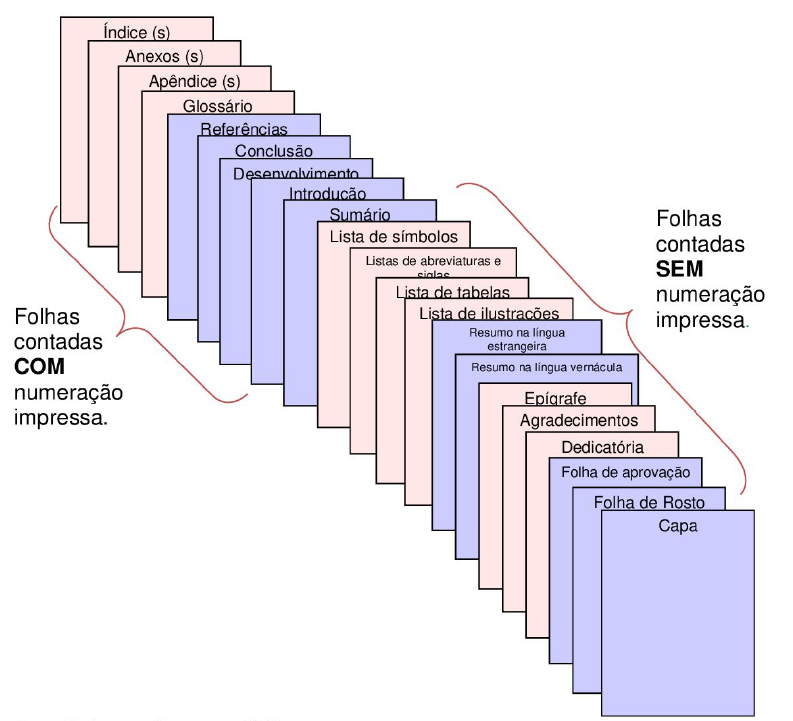
\includegraphics[width = 0.75\textwidth]{images/___fig1.png}
    \legend{\citeauthor{SIBI}}
\end{figure}

\section{Apresentação Gráfica Do Trabalho}
As orientações abaixo se referem a: trabalho de conclusão, monografias, dissertações e teses. Em alguns casos, são adequadas para uso na elaboração de relatórios de estágio, artigos e/ou \textit{paper} elaborados para entrega no IFC.


\subsection{Formato (tipo de papel, tamanho da fonte, margens)}


Apresentação gráfica de uma produção acadêmica a ser entregue na versão digital:

\begin{enumerate}[label=\alph*)]
   \item digitar o texto na cor preta. Cores somente em ilustrações como por exemplo: gráficos;
    \item  utilizar fonte tamanho 12 para o texto;
    \item  utilizar fonte tamanho 10 para citações longas, notas de rodapé, fontes (identificação) das ilustrações e tabelas e paginação;
    \item  optar por fontes arredondadas (\textit{Times New Roman} ou \textit{Arial}); 
    \item  margens:  superior de 3 cm;  inferior de 2 cm;  esquerda de 3 cm; direita de 2 cm.
    \item  inserir recuo de 2 cm, na primeira linha do parágrafo, a partir da margem esquerda;
    \item  inserir recuo de 4 cm, a partir da margem esquerda, na citação longa (com mais de três linhas);
    \item  digitar a nota de rodapé dentro das margens indicadas, devendo esta ficar separada do texto por um traço de 5 cm a partir da margem esquerda (ver seção 10);
    \item  apresentar o texto sobre a “natureza do trabalho” localizado  na folha de rosto e na folha de aprovação, a partir do meio da mancha gráfica para a margem direita (Figuras 12 e 15).
\end{enumerate}


Caso a produção acadêmica também seja entregue no formato impresso, observar os seguintes requisitos adicionais:

\begin{enumerate}[label=\alph*)]
    \item utilizar papel branco ou reciclado, formato A4 (21,0 x 29,7 cm);
    \item utilizar o anverso da folha para os elementos pré-textuais;
    \item poderá ser utilizado o anverso e verso da folha para impressão dos elementos textuais e pós-textuais;
    \item) adotar as margens:
\begin{table}[h!]
\centering
\begin{tabular}{|l|l|} 
\hline
\begin{tabular}[c]{@{}l@{}}- para o anverso da folha:\\-superior de 3 cm,\\-inferior de 2 cm,\\-esquerda de 3 cm,\\-direita de 2 cm.\end{tabular} & \begin{tabular}[c]{@{}l@{}}- para o verso:\\	-superior de 3 cm,\\	-inferior de 2 cm,\\-esquerda de 2 cm,\\	-direita de 3 cm.\end{tabular}  \\
\hline
\end{tabular}
\end{table}
\end{enumerate}


\subsection{Espaçamento}
O espaçamento que você deve adotar na formatação é:
\begin{enumerate}[label=\alph*)]
\item  espaço 1,5:
\begin{itemize}
\item[-] todo o texto;
\end{itemize}
\item um espaço de 1,5:
\begin{itemize}
\item[-] separa o texto da citação longa;
\item[-] separa cada título das seções e subseções do texto que os precede e que os sucede;
\end{itemize}
\item espaço simples para:
\begin{itemize}
\item[-] citações longas;
\item[-] notas de rodapé;
\item[-] referências;
\item[-] legenda e fonte das ilustrações e tabelas;
\item[-] natureza do trabalho;
\end{itemize}
\item um espaço simples:
\begin{itemize} 
\item[--] entre uma referência e outra, na lista de referências ao final do trabalho.
\end{itemize}
\end{enumerate}



\subsection{Indicativo de seção e numeração progressiva}
Seção é a divisão do TA, aplicada somente aos elementos textuais, que visa expor, numa sequência lógica, o relacionamento da matéria e permitir a sua localização. De acordo com a NBR 6024 \cite{abnt6024}, as seções também podem ser subdividas em subseções.
A seção primária é a principal divisão do texto do TA, que sempre deverá ser grafada em números inteiros a partir do 1, alinhados à esquerda por um espaço de caractere, e iniciar em página distinta e ímpar (anverso). As demais são chamadas de subseções e/ou seções secundária, terciária, quaternária e quinaria. Se for necessário enumerar os diversos assuntos de uma seção que não possua título, esta deve ser subdividida em alíneas. As alíneas são ordenadas alfabeticamente e terminam em ponto e vírgula, exceto a última, que termina em ponto. \textbf{Todas as seções devem conter um texto relacionado a elas e só devem ser subdivididas se houver necessidade de mais duas.}

Exemplo sugerido pelo IFC
\begin{itemize}
\item[] \textbf{1  SEÇÃO PRIMÁRIA (maiúsculas em negrito)}
\item[] 1.1  SEÇÃO SECUNDÁRIA (maiúsculas)
\item[] \textbf{1.1.1   Seção terciária (em negrito com primeira letra maiúscula)}
\item[] \textit{1.1.1.1 Seção quaternária (itálico com primeira letra maiúscula)}
\end{itemize}


\subsection{Paginação}
Para o TA, as páginas pré-textuais devem ser contadas, mas não numeradas. A contagem deve iniciar a partir da folha de rosto. Já a numeração propriamente deve aparecer somente a partir da primeira folha textual, em algarismos arábicos, e ser sequencial até o final do trabalho. 
O número da página deve aparecer no canto superior direito da folha, a 2 cm da borda, ficando o último algarismo a 2 cm da borda direita da folha.
A paginação da(s) referência(s), do(s) anexo(s) e do(s) apêndice(s) deve ser numerada sequencialmente no TA. As páginas que não permitem a inclusão de números também são contadas (mapas, documentos, ilustrações, etc.).
Para trabalhos com mais de um volume, a numeração sequencial das folhas deve ser mantida. Se o trabalho contiver apêndice e anexo, a numeração das páginas deve dar sequência ao texto principal.

\section{Ilustraçoes}
Independentemente do tipo de ilustração (quadro, desenho, figura, fotografia, mapa, entre outros), a sua identificação aparece na parte superior, precedida da palavra designativa. 
\begin{citacao}
Após a ilustração, na parte inferior, indicar a fonte consultada (elemento obrigatório, mesmo que seja produção do próprio autor), legenda, notas e outras informações necessárias à sua compreensão (se houver). A ilustração deve ser citada no texto e inserida o mais próximo possível do texto a que se refere. \cite[p. 11]{abnt14724}.
\end{citacao}

Um exemplo é apresentado na figura \ref{fig:fig2}:


\begin{figure}[!ht]
    \centering
    \caption{Modelo de gráfico}   \label{fig:fig2}
    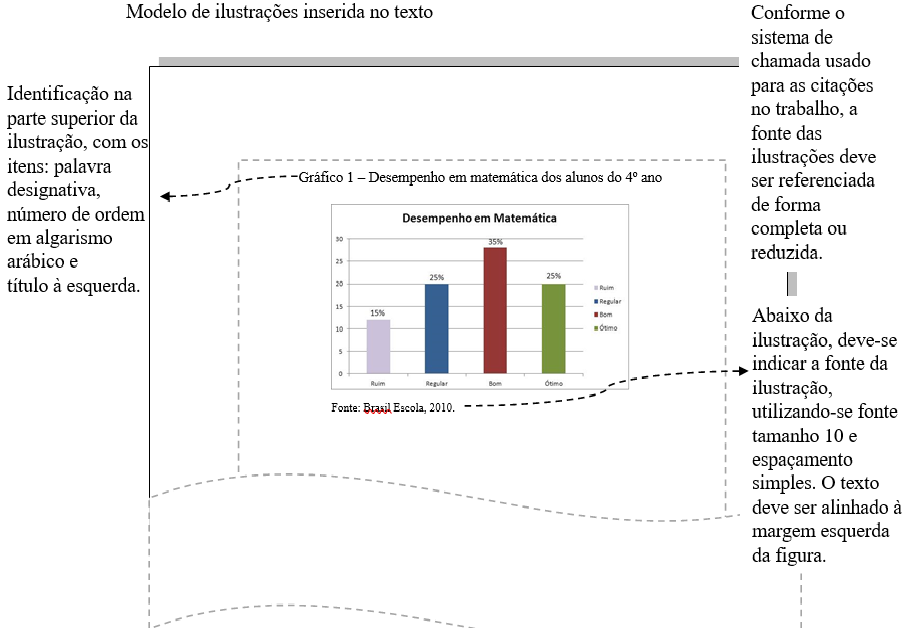
\includegraphics[width = 0.90\textwidth]{images/___fig2.png}
    \legend{\cite{SIBI}}
\end{figure}

\subsection{Equações e fórmulas}
As equações e fórmulas devem ser destacadas no texto para facilitar a leitura.  Para numerá-las, usar algarismos arábicos entre parênteses e alinhados à direita. Pode-se adotar uma entrelinha maior do que a usada no texto \cite{abnt14724}.
Exemplos são apresentados na equações \ref{eq:eq1} e \ref{eq:eq2}.

\begin{equation}
    \dot{x}(KT)\approx \frac{x(k+1)-x(k)}{T}
    \label{eq:eq1}
\end{equation}

\begin{equation}
    \frac{y(k)-y(k-1)}{T}+K\cdot y(t)=K\cdot u(t)
    \label{eq:eq2}
\end{equation}

\subsection{Tabela}

De acordo com Instituto Brasileiro de Geografia e Estatística (1993), tabela é uma forma não discursiva de apresentar informações em que os números representam a informação central. Um exemplo de tabela é encontrado na tabela \ref{tab:tab1}.
\begin{table}[h!]
\centering
\caption{Exemplo de tabela} \label{tab:tab1}
\begin{tabular}{llllllll} 
\hline
\multicolumn{8}{l}{Tabela de exemplo}  \\ 
\hline
aa & 1  & 0  & 0  & 0  & 0  & 0  & 0   \\ 
\hline
bb & zz & 2  & 0  & 0  & 0  & 0  & 0   \\ 
\hline
cc & zz & zz & 3  & 0  & 0  & 0  & 7   \\ 
\hline
dd & zz & zz & zz & 4  & zz & 6  & zz  \\ 
\hline
ee & zz & zz & zz & zz & 5  & zz & zz  \\
\hline
\end{tabular}
\end{table}

\chapter{\textbf{OUTRAS SEÇÕES}}

Este \textit{template} contém algumas seções criadas na tentativa de facilitar seu uso. No entanto, não há um limite máximo ou mínimo de seção a ser utilizado no trabalho. Cabe a cada autor definir a quantidade que melhor atenda à sua necessidade.
Um apêndice exemplo pode ser encontrado no apêndice \ref{Apend:Apend1} e um anexo exemplo pode ser encontrado no anexo \ref{Anex:Anex1}. 

\chapter{\textbf{MAIS SEÇÕES}}

Este \textit{template} contém algumas seções criadas na tentativa de facilitar seu uso. No entanto, não há um limite máximo ou mínimo de seção a ser utilizado no trabalho. Cabe a cada autor definir a quantidade que melhor atenda à sua necessidade. 

\chapter{\textbf{CONCLUSÃO}}

As conclusões devem responder às questões da pesquisa, em relação aos objetivos e às hipóteses/pressupostos. Devem ser breves, podendo apresentar recomendações e sugestões para trabalhos futuros.
%%%%%%%%%%%%%%%%%%%%%%%%%%%%%%%%%%%%%%%%%%%%%%%%%%%%%%%%%%%%%%%%%%%%%%%%%%%%%%%%%%%%%%%%%%%%%%%%
\postextual
\addtocontents{toc}{\protect\vspace{-\cftbeforechapterskip}}						% Manter esse comando para o espaçamento correto nas referências
\bibliography{ref.bib}
\begin{apendicesenv}
\chapter{Exemplo de Apêndice}

\label{Apend:Apend1}
Textos elaborados pelo autor, a fim de completar a sua argumentação. Deve ser precedido da palavra APÊNDICE, identificada por letras maiúsculas consecutivas, travessão e pelo respectivo título. Utilizam-se letras maiúsculas dobradas quando esgotadas as letras do alfabeto.

\end{apendicesenv}
\begin{anexosenv}

\chapter{Exemplo de Apêndice}
\label{Anex:Anex1}
São documentos não elaborados pelo autor que servem como fundamentação (mapas, leis, estatutos). Deve ser precedido da palavra ANEXO, identificada por letras maiúsculas consecutivas, travessão e pelo respectivo título. Utilizam-se letras maiúsculas dobradas quando esgotadas as letras do alfabeto.

\end{anexosenv}
%%%%%%%%%%%%%%%%%%%%%%%%%%%%%%%%%%%%%%%%%%%%%%%%%%%%%%%%%%%%%%%%%%%%%%%%%%%%%%%%%%%%%%%%%%%%%%%%

% \appendix

% \includepdf[
%     pages={1},angle=270,turn=false,noautoscale=true,fitpaper=true,frame=false,scale=0.8,
%     pagecommand={
%         \section{Lista de materiais}
%         \label{a:lista}
%     }
% ]{../calc.pdf}

%%%%%%%%%%%%%%%%%%%%%%%%%%%%%%%%%%%%%%%%%%%%%%%%%%%%%%%%%%%%%%%%%%%%%%%%%%%%%%%%%%%%%%%%%%%%%%%%
\end{document}
%%%%%%%%%%%%%%%%%%%%%%%%%%%%%%%%%%%%%%%%%%%%%%%%%%%%%%%%%%%%%%%%%%%%%%%%%%%%%%%%%%%%%%%%%%%%%%%%

% Exemplos:

% \begin{table}[!h]
%     \centering
%     \caption{Fatores de correção por circuito.}
%     \begin{tabular}{cC{2cm}C{2cm}C{2cmt}C{2cm}C{2cm}C{2cm}}
%         \hline
%         N & Potência (\si{\volt\ampere}) & Temperatura (\si{\celsius}) & Fator de correção de temperatura & Número de circuitos & Método de referência & Fator de correção de agrupamento \\
%         \hline
%         \hline
%         \openfile{../secao_projeto1.csv}
%         \tabularfromrange{1}{2}{7}{4}
%     \end{tabular}
%     \vspace{8pt}\\
%     \caption*{Fonte: Do autor.}
% \label{tab:secao_projeto1}
% \end{table}

% \begin{figure}[h!]
%     \centering
%     \caption{Gráfico de Torque e rendimento em função da velocidade de rotação do motor CC em ligação híbrida.}
%     \includegraphics[width=17cm]{imagens/2.3.eps}
% \label{fig:2.3}
% \end{figure}

% \begin{figure}[h!]
%     \centering
%     \caption{Circuito conversor proposto.}
%     \includesvg[width=14cm]{images/2.svg}
%     \label{fig:2.1}
% \end{figure}

% \begin{table}[!h]
%     \caption{Medição de grandezas para topologia de polarização como chave - Contatos do relé abertos e $R_b$ prático}
%     \centering
%     \begin{tabular}{|c|c|c|c|}
%         \hline % 
%         $R_{b}$ (\si{K\Omega}) & $i_{c}$ (\si{mA}) & $V_{ce}$ (\si{V}) & $V_{rele}$ (\si{V}) \\
%         \hline
%         \csvreader[head to column names]{exp4.3.csv}{}{ \rb & \ic   & \vce   & \vrele}
%         \\ \hline
%     \end{tabular}
% \end{table}

% \lstinputlisting[
%     language=Octave,
%     caption={"fir\_lowpass.m"},
%     label=code:fir_lowpass
% ]{../fir_lowpass.m}
